%%%%%%%%%%%%%%%%%%%%%%%%%%%%%%%%%%%%%%%%%%%%%%%%%%%%%%%%%%%%%%%%%%%%%%%%%%%%%%%%
%\documentclass[12pt,papel,twoside]{ibtesis}
\documentclass{ibtesis}

% \documentclass[12pt,papel,singlespace,oneside]{ibtesis}
% \documentclass[12pt,papel,preprint,singlespace,oneside]{ibtesis}

%%%%%%%%%%%%%%%%%%%%% Paquetes extra %%%%%%%%%%%%%%%%%%%%%%%%%%%%%%%%%%%%%%%%%%%
% Por conveniencia: aqu\'{\i} puede cargar todos los paquetes y definir los comandos 
% que necesite
\usepackage{ibextra}
\usepackage[utf8]{inputenc}
\usepackage{subcaption}  % Enable figure captions or figure notes
\usepackage{float}
\usepackage{nicefrac}
\usepackage{mathtools}
\usepackage{textcomp}
\usepackage[spanish]{babel}
\decimalpoint
\usepackage{amsfonts}

\newcommand{\done}{\item[\checkmark]}
%%%%%%%%%%%%%%%%%%%%%%%%%%%%%%%%%%%%%%%%%%%%%%%%%%%%%%%%%%%%%%%%%%%%%%%%%%%%%%%%
%%%%%%%%%%%%%%%%%%%%% Informacion sobre la tesis %%%%%%%%%%%%%%%%%%%%%%%%%%%%%%%

\title{Informe de Avance: Análisis de las direcciones de arribo de rayos cósmicos de ultra-alta energía en el Observatorio Pierre Auger}
\author{Evelyn~G.~Coronel}
\director{Dra.~Silvia Mollerach}

\carrera{Tesis de Maestría en Ciencias F\'{\i}sicas}
\grado{Maestrando}
\laboratorio{Partículas y Campos -- Centro At\'{o}mico Bariloche}
\jurado{Dr.~Diego~Harari (Instituto Balseiro)}

\palabrasclave{Rayos Cósmicos, Análisis de datos, Instituto Balseiro}
%\keywords{Cosmic Rays, Data Analysis, Balseiro Institute}
%\neembaeguasu{Mba'e michĩ yvágagui ouva, Mbo'ehaoguasu Balseiro}
% Si queremos poner la fecha manualmente:
% \date{Diciembre de 2099}

%%%%%%%%%%%%%%%%%%%%%%%%%%%%%%%%%%%%%%%%%%%%%%%%%%%%%%%%%%%%%%%%%%%%%%%%%%%%%%%%
%\titlepagefalse 
%%%%%%%%%%%%%%%%%%%%%%%%%%%%%%%%%%%%%%%%%%%%%%%%%%%%%%%%%%%%%%%%%%%%%%%%%%%%%%%%


% \setcounter{tocdepth}{4}
% \setcounter{secnumdepth}{4}
\begin{document}

\begin{preliminary}

%%% \'{I}ndices %%%%

\begin{abreviaturas}

\begin{tabular}{l l}
CR: 		& Rayos cósmicos  (\emph{Cosmic Rays}) \\
SD: 		& Detector de Superficie (\emph{Surface Detector})  \\
EAS: 		& Lluvia Atmosférica Extendida  (\emph{Extensive Air Shower})    \\
S(1000): 	& Señal a 1000\,m del núcleo de la lluvia y al nivel del suelo \\
S(1000)$_w$:& Señal de S(1000) corregida por la modulación del clima. \\
S$_{38}$: 	& Señal a 1000\,m del núcleo y al nivel del suelo si el ángulo cenital del evento fuera de $38^o$\\
S$_{38,w}$: & Señal S$_{38}$ corregida por la modulación del clima \\
eV: 		& electrón Voltio, $1\,$eV$= 1.602\times 10^{-19}\,$J \\
EeV: 		& $1\,$EeV$=10^{18}\,$eV\\
ICRC: 		& Conferencia Internacional de Rayos Cósmicos (\emph{International Cosmic Ray Conference})\\
\end{tabular}
                     %Abreviaturas
\end{abreviaturas}

	\tableofcontents                %\'{I}ndice
	\listoffigures                  %Figuras
	%\listoftables                  %Tablas

	%\begin{resumen}%
Cuando un rayo cósmico interactúa con una molécula en la parte superior de la atmósfera, se inicia un proceso en el cual se generan otras partículas secundarias. Este proceso es conocido como lluvia atmosférica extendida. Estas lluvias pueden ser detectadas sobre la superficie de la Tierra mediante varios experimentos. Este trabajo utiliza los datos recolectados por los detectores de superficie separados en 1500\,m entre sí del Observatorio Pierre Auger durante los años 2005-2020. 

Se estudian eventos obtenidos mediante distintos algoritmos de adquisición de datos. El \emph{Disparo Estándar} que alcanza eficiencia completa para eventos asociados a rayos cósmicos de energía mayor a $3\,$EeV, y el \emph{Todos los Disparos} llega a detectar, con una eficiencia del 100\%, eventos por encima de $1\,$EeV. El primer disparo contiene eventos registrados desde el año 2005 y el segundo disparo empezó funcionar desde el 2013. 

Las condiciones atmosféricas como la presión (P), la temperatura (T) y la densidad ($\rho \propto \nicefrac{P}{T}$) afectan el desarrollo de la lluvia a través de la atmósfera. Las variaciones de estas condiciones inducen una modulación en la señal producida en los detectores por un rayo cósmico de una dada energía. Mediante un estudio hecho por la Colaboración sobre eventos del Disparo Estándar, se corrigió el efecto de esta modulación en la estimación de la energía de los rayos cósmicos medidos por el Observatorio. En este trabajo extendimos el periodo de tiempo analizado de esta modulación, y se observó que los parámetros obtenidos son comparables con la reconstrucción oficial. También se estudia la modulación en los datos de Todos los Disparos, y se realiza una corrección sobre el mismo conjunto de datos usando los parámetros obtenidos por este trabajo.

Se  estudian las modulaciones en distintas frecuencias mediante el análisis en Rayleigh, y se propone una variable generalizada para hacer un barrido en frecuencias con el método de East-West. Se obtienen resultados de la modulación en ascensión recta para distintos rangos de energía y se comparan con resultados reportados por la Colaboración Pierre Auger.

\end{resumen}


% \begin{nemombyky}%
% Mbyjakua\'ape (\emph{astronomía} karaiñe'\~eme) ojeikuaase mba\textquotesingle e oik\'ova umi mba\textquotesingle e  michĩ yv\'agagui o\'uva (\emph{rayos cósmicos} karaiñe'\~eme) oguah\~evove amo yvatetépe (\emph{atmósfera} karaiñe'\~eme). Ombok\'aramo tuminguaave\textquotesingle \~yty (\emph{conjunto de átomos o molécula}  karaiñe'\~eme ) yvatetépe oĩva, oñepyr\~u ojapo het\~a umi tuminguaave\textquotesingle \~yjokaku\'era (\emph{partículas}  karaiñe'\~eme ) op\'arupi. Ko\textquotesingle a       ha\textquotesingle e  h\'ina peteĩ ama guasu tuminguaave\textquotesingle \~yjoka rehegua ( \emph{lluvia atmosf\'erica extendida} karaiñe'\~eme). Umi ama guasuku\'era tuichaterei ha ikatu eñeña\textquotesingle ã yvy ári op\'arupi. Mend\'osape oĩ peteĩ mba\textquotesingle etuicha h\'erava \emph{Pierre Auger} Mbyjañama\textquotesingle \~eha\~gua (\emph{Observatorio Pierre Auger}) oña'\~ava ko ama. Ko\textquotesingle  ape romba\textquotesingle  ap\'ota umi ama ko mbyjañama\textquotesingle \~eha\~gua oña\textquotesingle \~ava\textquotesingle  kue 2005-guive 2018-peve. Mba\textquotesingle \'eichapa umi amaku\'era oguah\~e yvy \'ari ikatu ojuavy hakúramo (T, \emph{temperatura} karaiñe\textquotesingle \~eme) tér\~a  poh\'yiramo pe pytundyry mbyjañama\textquotesingle \~eha\~gua áripe ($\rho$, \emph{densidad} h\'erava karaiñe\textquotesingle \~eme). Ko mbyjañama'\~eha\~gua ojapova\textquotesingle ekue peteĩ tembiapo ha ko\textquotesingle ape rojapojey up\'eva roikuaaha\~gua umi papapo oñenoh\~eva\textquotesingle ekue oiko gueteri ko'\~anga peve, ha rotopa kóva oikópa añetete.
% \end{nemombyky}



%%% Local Variables: 
%%% mode: latex
%%% TeX-master: "template"
%%% End: 


\end{preliminary}


\chapter{Introducción}
\graphicspath{{0_Introduccion/}}
% INTRODUCCION

La parte superior de la atmósfera terrestre está siendo constantemente bombardeada con partículas provenientes del espacio, con energías de los $10^{10}\,$eV para arriba. Estas partículas son conocidas como rayos cósmicos (RC) y han sido medidas desde los años 60s \cite{linsley1961extremely}. Aunque el área lleva tiempo siendo estudiada, los mecanismos que producen los RCs y las zonas del espacio donde se originan los mismos siguen siendo investigadas por distintos experimentos. 


Por encima de una energía de $10^{14}\,$eV, los RCs que llegan a la atmósfera pueden interactuar con las moléculas de la misma,  y así producir cascadas de partículas secundarias. Dependiendo de la energía del primario, es decir el RC que generó la lluvia, estas partículas pueden ser medidas usando detectores sobre la superficie de la Tierra. Esta cascada es conocida como lluvia atmosférica extendida o \emph{EAS} y está compuesta por una componente electromagnética, que consiste en electrones, positrones y fotones, y una componente muónica. Las partículas secundarias cargadas también pueden excitar moléculas de nitrógeno en el aire que producen fotones de fluorescencia y pueden ser observados por telescopios durante noches claras.


El observatorio Pierre Auger está ubicado en la ciudad de Malargüe, provincia de Mendoza. El mismo fue construido para detectar las partículas secundarias de las EASs producidas por RCs, con energía por encima de $0.1\,$EeV. La adquisición de datos empezó en el año 2004. El observatorio posee un sistema híbrido de detección, ya que combina un arreglo de detectores de partículas sobre la superficie y un conjunto de telescopios que detectan los fotones de fluorescencia. Cuando el observatorio  registra una EAS que llega a la superficie y reconstruye la dirección de llegada del RC, se dice que se ha detectado un \textit{evento}.


Los análisis presentados en este trabajo fueron realizados con los eventos obtenidos por $\sim 1600$ detectores Cherenkov, dispuestos sobre de $\sim 3000\,\text{km}^2$ a  $1500\,$m entre sí. Un conjunto de 7 detectores adyacentes, es decir una en el medio y 6 en los lados, forman una celda hexagonal. Esta disposición de tanques se menciona como \textit{arreglo principal}.   Cada detector consiste en un tanque cilíndrico con 12 toneladas de agua ultra-pura de $1.2\,$m de alto. En la parte superior del tanque están instalados 3 foto-multiplicadores que monitorean la radiación Cherenkov en el agua. El conjunto del tanque y la electrónica de detección  se menciona durante este trabajo como \textit{Surface Detector} o \textit{SD}.  Cada detector está midiendo constantemente los fotones en el agua. Muchos de estos fotones son producidos por ruido y otros por partículas secundarias de una EAS. Los SDs cuentan con algoritmos o reglas para discernir ruido de un evento causado por un rayo cósmico, estos son los algoritmos de disparo.


\section{Acerca de todos los disparos del SD}

A medida que los tanques pasan más tiempo midiendo, también van perdiendo sensibilidad a los eventos de bajas energías. Esto es una desventaja del disparo estándar en los SDs en el rango $1\,$EeV - $2\,$EeV, ya que la eficiencia completa  del disparo estándar se obtiene para eventos de energía mayor a $2.5\,$EeV.  En la Fig.\ref{fig:futuro}, para los datos presentados en el ICRC 2019, se observa como la energía media de los eventos para distintos rangos de tiempo va aumentando, además que la proporción de eventos por debajo de $3\,$ EeV disminuye. 

\begin{figure}[H]
	\centering
	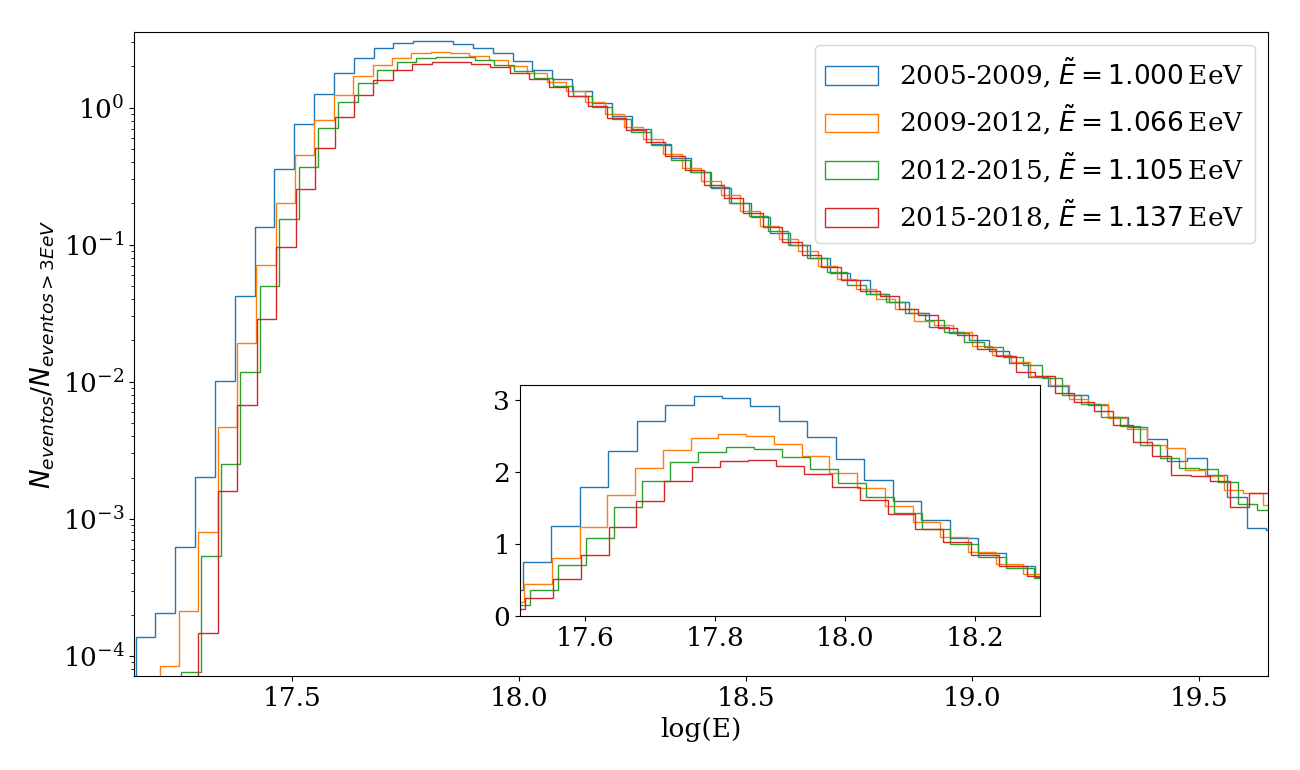
\includegraphics[width=0.8\textwidth]{histograma_evolucion_eventos.png}
	\caption{Histograma de eventos  del Disparo Estándar por rango de tiempo medido por el Observatorio Pierre Auger}
	\label{fig:futuro}
\end{figure}

\begin{figure}[H]
	\centering
	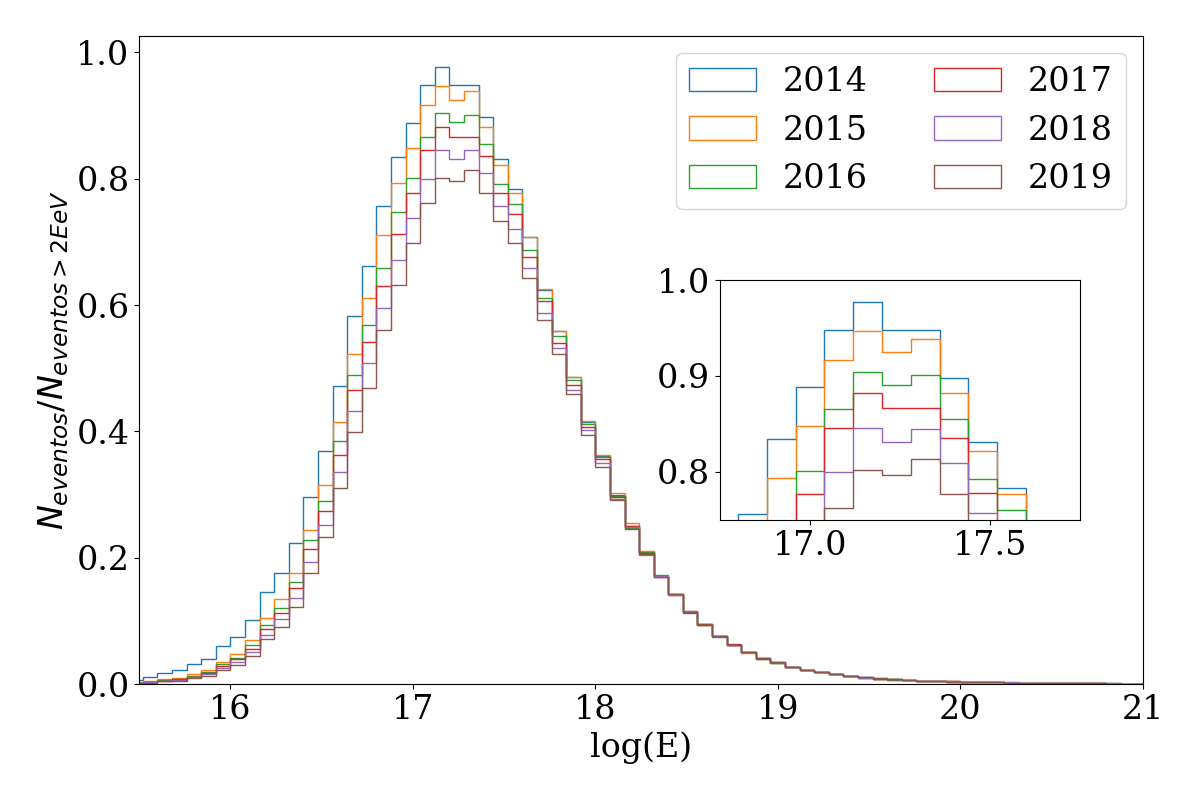
\includegraphics[width=0.8\textwidth]{figura_harari.png}
	\caption{Histograma de eventos de  Todos Los Disparos por rango de tiempo medido por el Observatorio Pierre Auger}
	\label{fig:TLD}
\end{figure}


El análisis del trabajo de licenciatura fue realizado sobre los eventos medidos utilizando el disparo estándar del arreglo principal, cuya eficiencia varía con la energía del CR. Para el disparo estándar, los eventos con energía mayor a $3\,$EeV y ángulo cenital $\theta<60^o$ o  por encima de $4\,$EeV y $\theta<80^o$, son detectados con una eficiencia del 100\%. Por lo tanto, el análisis en el rango de energía entre $1\,$EeV - $2\,$EeV requiere factores relacionados con la eficiencia del disparo en función de la energía. Estos factores son obtenidos de manera fenomenológica \cite{taborda}. 

Para superar esta dificultad y  poder recuperar la sensibilidad para bajas energías, a partir del año 2013  se implementó otros algoritmos de disparo en los SDs, llamados ToTd y MoPS \cite{pierre2013plans}. Estos algoritmos de disparo se mencionan en este trabajo como \textit{todos los disparos}. 

La implementación de los ToTd y MoPS fue llevada a cabo mediante una actualización de la electrónica de los SDs para bajar el umbral de disparo, en particular para las señales de la componente electromagnética de la EAS, mejorando así la reconstrucción de eventos mediante la separación fotón/hadrón para bajas energías  \cite{pierre2013plans}. Con esta mejora, el umbral de eficiencia completa para todos los disparos es menor que el disparo estándar, este umbral es de una energía de $1\,$EeV. En la Fig\,\ref{fig:triggers} se comparan las eficiencia del disparo estándar y todos los disparos en función de la energía del evento. De tal manera que, al estudiar los eventos en el rango $1\,$EeV - $2\,$EeV,  no son necesarios los factores de eficiencia y sólo pueden afectar los cambios de la exposición direccional del observatorio.


\begin{figure}[H]
  \centering
  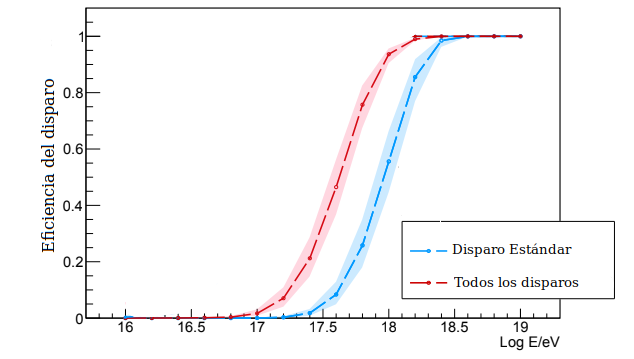
\includegraphics[width=0.75\textwidth]{comparacion_triggers.png}
  \caption{La eficiencia del disparo en función de la energía para eventos con ángulo cenital $\theta$ menor a $60^o$. Este figura fue extraída del trabajo \cite{triggers_ref}}
  \label{fig:triggers}
\end{figure}


Una desventaja de todos los disparos sobre el disparo estándar, es que el último tiene una mayor cantidad de años medidos, ya que se adquieren datos  desde el año 2004 con este algoritmo. Esto es conveniente ya que mientras más años han sido medidos es más factible que los efectos espúreos se cancelen. En cambio, para todos los disparos, el análisis  es posible desde el año 2013. Entre inicios del 2004 y finales del 2019, el conjunto de eventos del disparo estándar tiene $6\,975\,194$ eventos sin clasificar, es decir todos los eventos registrados por el observatorio sin discriminar por energía. En cambio entre mediados del 2013 hasta fines del 2019, el archivo de eventos para todos los disparos tiene $13\,739\,351$ eventos sin clasificar, por lo que el menor tiempo de medición se compensa con la eficiencia del disparo.


\section{Acerca de los eventos} \label{filtro}

Se aplican cortes a los eventos para asegurar la eficiencia completa de los detectores. Estos cortes implican límites en ángulo cenital $\theta$ de los eventos, en la cantidad de vecinos al tanque de mayor señal, además de restringirse a eventos medidos en condiciones normales, es decir, cuando los sistemas de comunicación del Observatorio funcionan sin inconvenientes. De esta manera, podemos prescindir de otros factores de corrección.

A partir de los registros de eventos del arreglo principal con todos los disparos, se consideran solamente los eventos que cumplan las siguientes características:

    \begin{enumerate}
      \item La calidad de la reconstrucción depende de la energía y del ángulo cenital $\theta$ del evento.  Para el disparo estándar los eventos por debajo de los $4\,$EeV, se consideran los eventos con $\theta < 60^o$, en cambio para eventos por encima de esta energía se consideran hasta $\theta < 80^o$. Para todos los disparos se consideran solo los eventos con $\theta<60^o$.
      \item Los datos del evento son recopilados sin inconvenientes. Este filtro se conoce como \emph{Bad period flag} o $ib$. Un valor de 1 indica un buen periodo. Con este filtro se descartan eventos debido a probables fallas de alimentación o problemas de comunicación o adquisición que podrían inducir errores en el análisis.
      \item Buena reconstrucción de la lluvia atmosférica asociada al evento.
      \item El tanque de mayor señal está en el interior de un hexágono de tanques activos. Estos eventos se conocen como \textit{eventos 6T5}.
    \end{enumerate}


\subsection{Acerca del registro de hexágonos}\label{hexagonos_rate}

La cantidad de celdas  activas sobre el observatorio está relacionado con el filtro de eventos $6T5$, que garantiza la calidad de la reconstrucción del evento. El observatorio lleva un registro de la cantidad de hexágonos activos cada 5 min, además de registrar las condiciones atmosféricas en distintas estaciones de clima sobre la superficie del observatorio. 


\section{Acerca de la tesis de licenciatura}

Durante la tesis de licenciatura se analizaron los efectos de las condiciones atmosféricas durante el desarrollo de las EAS.  Se analizaron los datos adquiridos durante en el periodo 2005-2018 por el arreglo principal. De esta manera, se extendió los periodos estudiados anteriormente en los siguientes trabajos \cite{abraham2009atmospheric}, \cite{abreu2012description}   y \cite{aab2017impact}. 

Los efectos atmosféricos afectan principalmente a la atenuación de la componente electromagnética  de la EAS, en particular depende fuertemente de la temperatura y presión. Estos efectos  se caracterizan por parámetros dependientes del ángulo cenital del evento y por la presión, densidad y temperatura al momento de su detección. Los parámetros mencionados se utilizan para corregir las señales registradas por los SDs. Las correcciones del clima utilizadas por la colaboración Pierre Auger fueron implementadas a partir del trabajo \cite{aab2017impact} en el 2017. 

Durante el trabajo de la licenciatura se reprodujo el análisis de la modulación del clima sobre el periodo 2005-2015 del trabajo \cite{aab2017impact}, obteniéndose resultados compatibles. También se estudió la modulación del clima mediante el valor de la señal medida por los SDs, $S_{38}$, sin la corrección propuesta por \cite{aab2017impact}, además de extender el rango de tiempo analizado hasta el 2018. Se observó que los parámetros del clima obtenidos en este análisis sobre  $S_{38}$  son compatibles con los utilizados en la reconstrucción oficial. 


\chapter{Métodos}
\graphicspath{{1_Metodo/}}
% METODOS
El estudio de la distribución de las direcciones de arribo de los eventos es una herramienta importante para obtener información sobre el origen de los RCs . Las irregularidades sobre el flujo casi isotrópico de los RCs, en un rango de energía, pueden deberse a  zonas del espacio donde se producen más RCs que en otras, estas irregularidades se conocen como anisotropías. 

El análisis de anisotropías a grandes escalas angulares suele ser hecho sobre las irregularidades de la distribución de eventos en ascensión recta $\alpha$, ya que el arreglo principal tiene una exposición direccional en función de esta coordenada casi constante \cite{referencia_anis}.

\section{Cálculo de los coeficientes de Fourier para el análisis de anisotropía en ascensión recta}

Las anisotropías son variaciones pequeñas por lo que eliminar todo factor espurio en el análisis es importante. Para obtener la amplitud de la misma en ascensión recta, se estudia la frecuencia sidérea ($f_{sid}=366.25\,$ ciclos/año) \cite{taborda}. Los errores sistemáticos debido a la modulación de eventos por el clima u otros errores propios de la adquisición de datos, aparecen en la frecuencia solar  ($f_{sid}=365.25\,$ ciclos/año), por lo que se debe tener en consideración el análisis de esta frecuencia. La frecuencia anti-sidérea ($f_a=364.25\,$ ciclos/año) es una frecuencia que puede indicar efectos sistemáticos en la amplitud de la anisotropía en la frecuencia sidérea \cite{farley1954sidereal}. La mezcla entre modulaciones diarias y anuales induce bandas laterales ubicadas a $\pm1\,$ciclo/año con respecto a la solar \cite{taborda}. Por estos motivos se toman estas frecuencias  como referencia.

  \subsection{Variaciones relativas de los hexágonos} \label{peso_hexagonos}

Para corregir las variaciones de la exposición del observatorio, podemos definir un peso  $w_i$ por cada evento $i$, que corrige la variación  $\Delta N_{cell}(\alpha^0)$ en función de la ascensión recta del cenit del observatorio $\alpha^0$ durante el rango de tiempo estudiado. Estas variaciones pueden deberse al crecimiento del arreglo a través de los años,  por caídas en la comunicación del observatorio con los SDs u otros motivos. 

El factor $\Delta N _{cell}(\alpha^0)$ tiene en cuenta que la exposición  direccional  el observatorio no es uniforme en tiempo sidéreo.  Se obtiene sumando el número de celdas durante el periodo de medición, en cada segmento de $\alpha^0$ y luego se normaliza con el valor medio de los segmentos.

Para calcular estos pesos $w_i$, se sigue el algoritmo presentado a continuación:
     
      \begin{enumerate}
        \item Se establecen una frecuencia $f$  y un rango de tiempo a estudiar. Por ejemplo, se desea estudiar la frecuencia solar entre el 1 de Enero del 2014 a las 12:00:00 GMT y el 1 de Enero del 2020 a las 12:00:00 GMT.

        \item Cada dato del registro de hexágonos, tomado en un momento $t$ durante el rango seleccionado, se clasifica según la cantidad de horas desde un momento de referencia $t_0$. Esta referencia $t_0$ se tomará como el 1 de Enero del 2005 a las 00:00:00 GMT, o  $21\,$hs del 31 de Diciembre del 2004, según la hora local de Malargüe.

        \item Podemos asociar una coordenada angular $h$ a $t$  y $f$  utilizando la siguiente expresión:
         \begin{equation}
          h = (t-t_0) \times \frac{360^o}{24\text{hs}} \times\frac{f}{f_{Solar}} + h_0
          \label{eq:h_horas} 
        \end{equation}
        El factor $\nicefrac{f}{f_{Solar}}$ sirve para hacer un cambio de escala temporal entre los periodos de distintas frecuencias. Se usa como referencia la $f_{Solar}$ dado que las horas (solares) se basan en esta frecuencia, y el valor de $h_0=31.4971^o$ representa la ascensión recta del cenit del observatorio en el momento utilizado como referencia.
        
        \item  Para simplificar el cálculo del peso de los hexágonos, se divide los $360^o$ de la ascensión recta en $L$ segmentos de $\nicefrac{360}{L} ^o$ cada uno. Para clasificar un dato se  toma  el valor $h$  y se calcula
        \begin{equation}
          h' = h\, mod \,360 %=  h - 360\Big \lfloor \frac{h}{360} \Big \rfloor
          \label{eq:h_primado}
        \end{equation}
        donde la función $mod$ representa la función módulo que devuelve un número real positivo. Con el valor de $h'$ del dato, se asigna el mismo al segmento $k$ que le corresponde, mediante la siguiente expresión
        \begin{equation}
          k = \bigg \lceil \frac{h'}{360}\times L \bigg \rceil
        \end{equation}
        donde $\lceil a \rceil$ representa la función techo \footnote{La función techo da como resultado el número entero más próximo por exceso}. Por ejemplo, si optamos por $L=24$ y un dato en particular resulta con  $h=395\,^o$, esto implica que $h'= 35^o$ y que $k=\lceil 2.333 \rceil=3$, por lo tanto, este registro corresponde al segmento en la $3^{a}$ posición.

        \item Una vez clasificados todos los datos del registro de hexágonos, se calcula la suma  $N_{hex, j}$ de los datos que cayeron un segmento $j$ dado. Para definir la variación relativa de hexágonos  $\Delta N_{cell,k}$ de un segmento $k$ en particular, necesitamos la media de hexágonos por segmento $ \langle N \rangle$  para normalizar las variaciones.
       \begin{align}
         \langle N \rangle &= \sum^{L}_{i=1} \frac{N_{cell, i}}{L}  \qquad
         \Delta N_{cell,k} = \frac{N_{cell, k}}{\langle N \rangle}  \label{epepe}
       \end{align}

      \end{enumerate}
 En la Fig.\ref{fig:pesos_referencia} se muestran las variaciones relativas de los hexágonos en función de la ascensión recta del cenit del observatorio para las frecuencias mencionadas. Este análisis fue realizado en el marco del trabajo \cite{referencia_pesos} con eventos del periodo 2004-2017. 



       En la Fig.\ref{fig:pesos_ejemplo} se observan los valores obtenidos de $\Delta N_{cell,k}$  con el código escrito para este trabajo, en función de la ascensión recta del cenit  para $L=288$ segmentos. Se analizó el conjunto de datos  utilizado para obtener los resultados la Fig.\ref{fig:pesos_referencia}, con el fin de validar dicho código. Los datos se analizaron desde el 1 de Enero del 2004 a las 00:00:00 GMT  hasta el 1 de Enero del 2017 a las 00:00:00 GMT. Se  observa que estos los resultados obtenidos son compatibles con la Fig.\ref{fig:pesos_referencia}
      
      \begin{figure}[H]
          \centering
              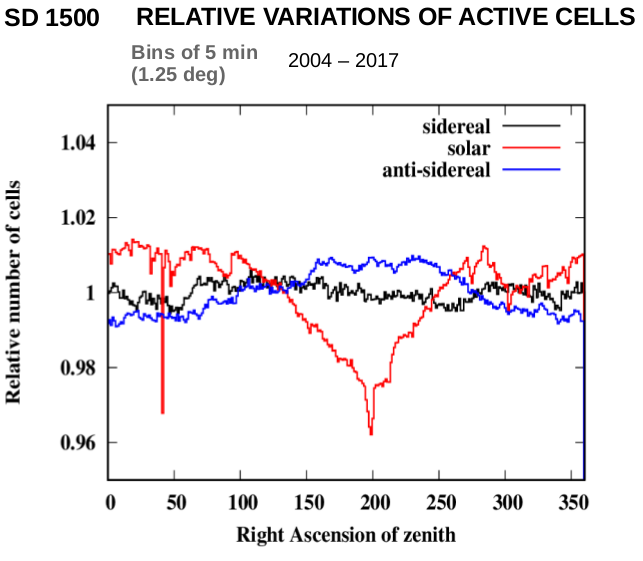
\includegraphics[width=0.5\linewidth]{pesos_referencia.png}  
              \caption{Valores de $\Delta N_{cell, k}$ en el rango 2004-2017 para distintas frecuencias obtenidas en el trabajo \cite{referencia_pesos}.}
              \label{fig:pesos_referencia}
        \end{figure}

       \begin{figure}[H]
          \centering
              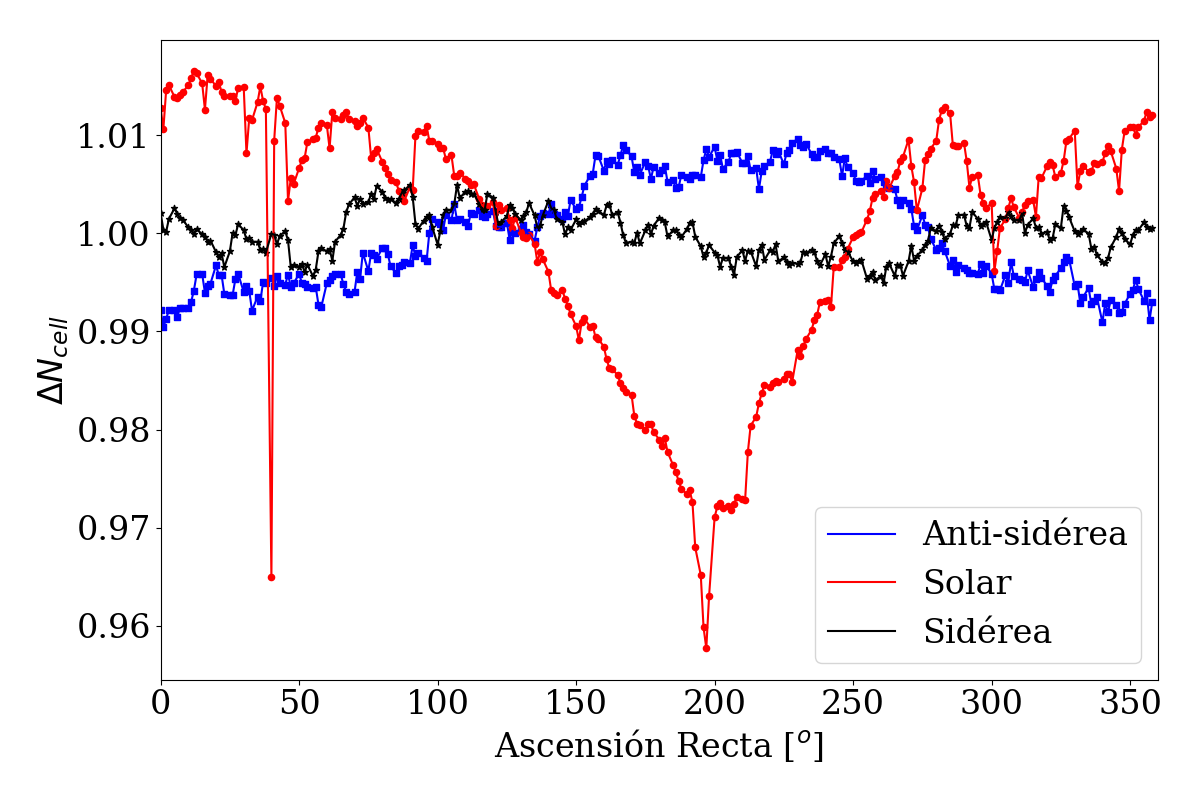
\includegraphics[width=0.75\linewidth]{weigths_2020.png}
              \caption{Valores de $\Delta N_{cell, k}$ en el rango 2004-2017 para distintas frecuencias utilizando el código escrito en este trabajo.}
              \label{fig:pesos_ejemplo}
        \end{figure}

    Para una representación fiel entre los registros de los hexágonos y los pesos de los eventos, se optó por clasificar los datos de los hexágonos en $288$ segmentos, donde cada segmento tiene un ancho de $1.25^o$. Esto es conveniente ya que la actualización del registro de hexágonos se realiza una vez  cada $5\,$min como se menciona en la sección \ref{hexagonos_rate}. Esta tasa de actualización es equivalente a decir que la adquisición se realiza cada vez que el cenit del observatorio barre  $1.25^o$ en ascensión recta sobre la esfera celeste.


  \subsection{Cálculo de Rayleigh en ascensión recta para una frecuencia dada} \label{rayleigh}

  Un procedimiento para estudiar anisotropías en la direcciones de arribos de los RCs es realizar un análisis de Fourier en ascensión recta $\alpha$. La distribución en ascensión recta $\alpha$ del flujo de RCs $I(\alpha)$ que llega al arreglo principal puede caracterizarse por las amplitudes $r_k$ y fases $\phi_k$ de su expansión en serie de Fourier al $k-$ésimo orden. 

  \begin{equation}
    I(\alpha) = I_0 \bigg ( 1+ \sum^\infty_{k=1} r_k\cos{[k(\alpha - \phi_k)]} \bigg) = I_0 \bigg ( 1+ \sum^\infty_{k=1} a_k\cos{k\alpha} +  b_k\sin{k\alpha} \bigg ) 
  \end{equation}
  donde $a_k=r_k\cos k\phi_k$ y $b_k=r_k\sin k \phi_k$, y $I_0$ es el flujo medio. La distribución $I(\alpha)$ puede obtenerse a partir de la distribución de direcciones de arribo de los eventos observados.  En este trabajo, suponiendo que existieron $N$ eventos en el rango analizado, se considera que los mismos tienen una distribución en ascensión recta del tipo $\nicefrac{dN}{d\alpha}= \sum^N_{i=1} \delta(\alpha - \alpha_i)$ \cite{taborda}. 

  Como se mencionó anteriormente, los análisis en ascensión recta están asociados a la frecuencia sidérea. Para realizar el análisis de los eventos en cualquier frecuencia arbitraria, es necesario modificar $\alpha$ por $\tilde{\alpha}$. Esta nueva variable tiene la forma como se utiliza en el trabajo \cite{taborda}:
  \begin{equation}
    \tilde{\alpha} = 2\pi f_x t_i + \alpha_i - \alpha_i^0(t_i) \label{ra_mod}
  \end{equation}
  donde $f_x$ es el frecuencia arbitraria a estudiar, $t_i$ es el momento en que ocurrió el evento y $\alpha_i^0(t_i)$ es la ascensión recta del cenit del observatorio en el momento del evento. Si la frecuencia a analizar es la sidérea, el análisis con $\alpha$ y $\tilde{\alpha}$ arrojan los mismos parámetros $r_k$ y $\phi_k$.

 Clasificando a los eventos mencionados en la sección \ref{specs} según el valor de la ascensión recta y considerando que todos los eventos tienen un peso uniforme de $w_i=1$, se dicen que los eventos fueron analizados \textit{sin pesos}, donde no consideramos la corrección de la exposición. En caso contrario, se habla de análisis \textit{con pesos} de los hexágonos  y estos pesos se calculan como se menciona en la sección anterior.

  Para realizar el análisis de frecuencias de los eventos, en el $k$-ésimo orden en la expansión de Fourier, se siguen los siguientes pasos.

        \begin{enumerate}
        \item Fijando un rango de tiempo y un rango de energía en el cual se desea estudiar la anisotropía, se establece una frecuencia en particular $f$ a analizar. Siguiendo el ejemplo de la sección anterior, se analiza la frecuencia solar entre el 1 de Enero del 2014 a las 12:00:00 GMT y 2019 hasta el 1 de Enero del 2020 a las 12:00:00 GMT.

        \item Con los eventos ya filtrados según el criterio de la sección \ref{filtro}, asigno cada evento $i$ un valor $h_i$, definida en la Ec.\ref{eq:h_horas}

        \item En caso de considerar los pesos de los hexágonos, para asignar el peso correspondiente al evento, se asocia a un segmento $k$, calculado en la sección \ref{peso_hexagonos}, mediante el valor de $h'_i$ definido en la Ec.\,\ref{eq:h_primado}. Luego, el peso asignado $w_i$  al evento $i$ es: $ w_{i}= (\Delta N_{cell,k})^{-1}$, caso contrario, se toman que todos los eventos tiene $w_i=1$.
        
        \item Para el análisis en frecuencias, a partir del valor de $h_i$ se asigna el ángulo $\tilde{\alpha}_i$ definida en la Ec.\ref{ra_mod}. La implementación en el código es de la siguiente manera: 
        \begin{equation}
         \tilde{\alpha}_i = 2\pi \frac{h_i}{24} + \alpha_i -\alpha^0_{i}
        \end{equation}
        donde $\alpha_i$  representa la ascensión recta del evento y $\alpha^0_{,i}$ la ascensión recta en el cenit del observatorio en el momento del evento. Cabe resaltar que la información de la frecuencia que se está estudiando se encuentra en el valor de $h$. Si la frecuencia a estudiar fuera la sidérea, el término $2\pi \frac{h}{24} $ seguiría el cenit del observatorio, por lo que este término sería equivalente a $\alpha^0_{i}$, por lo tanto en esta frecuencia $ \tilde{\alpha}_i =\alpha_i$ como es de esperarse. 
        
        \item Para calcular los coeficientes de Fourier del k-ésimo armónico $a_k$ y $b_k$, se siguen los siguiente pasos:
        \begin{enumerate}
          \item Por cada evento  $i$ se calculan los siguientes valores:
          \begin{equation}
             a_{ik}' = {w_i}\cos k\tilde{\alpha}_i \qquad
             b_{ik}' = {w_i}\sin k\tilde{\alpha}_i
         \end{equation}
         \item Una vez que se obtuvieron los valores de $a_{ik}'$ y $b_{ik}'$ para todos los eventos en el rango de tiempo estudiado, se calculan los coeficientes definidos en el trabajo \cite{analisis_fourier} mediante:
         \begin{alignat}{3}
          \mathcal{N} &= \sum^{Eventos}_i w_i \qquad
            a_k = \frac{2}{\mathcal{N}} \sum^{Eventos}_i a_{ik}' \qquad
            b_k = \frac{2}{\mathcal{N}} \sum^{Eventos}_i b_{ik}'  
         \end{alignat}
        \end{enumerate}
        \item Con los coeficientes es posible calcular la amplitud de la frecuencia estudiada $\tilde{r}$ y la fase $\phi$. Otros parámetros calculados para el análisis son la probabilidad $P(\tilde{r})$  y $r_{99}$. 
        \begin{alignat}{3}
            \tilde{r}_k &= \sqrt{a_k^2 +b_k^2}                       \qquad &&   \phi_k&&= \frac{1}{k}\arctan\frac{a_k}{b_k}\\
          P(\tilde{r}_k)&= \exp(-\mathcal{N}\frac{\tilde{r}_k^2}{4})\qquad &&   r_{99}&&= \sqrt{\frac{-4\log(0.01)}{\mathcal{N}}}
        \end{alignat}
        Cabe resaltar que el $r_{99}$ depende solamente de los pesos de los eventos que se está estudiando. La interpretación  de este valor es cual es la probabilidad de tener una amplitud mayor como una fluctuación de una distribución isotrópica sea del $1$\%
        %., y el valor de amplitud $r_{99}$ para que dicha probabilidad sea del $1$\%.
      \end{enumerate}

    Una forma de validar el código para el análisis de anisotropía es comparar los resultados del código con los obtenidos en otros trabajos \cite{taborda}. En la Fig.\ref{fig:sin_pesos_referencia} se muestra el análisis hecho sobre el mismo conjunto de eventos. Estos eventos fueron adquiridos con el disparo estándar desde el 1 de Enero del 2004 a las 00:00:00 GMT  hasta el 1 de Enero del 2017 a las 00:00:00 GMT. Se consideraron los eventos por encima de $8\,$EeV que además cumplan las condiciones dadas en la sección \ref{filtro}.  En esta figura que los resultados obtenidos en \cite{taborda} y con el código utilizado por este trabajo son indistinguibles. 

      \begin{figure}[H]
        \centering
        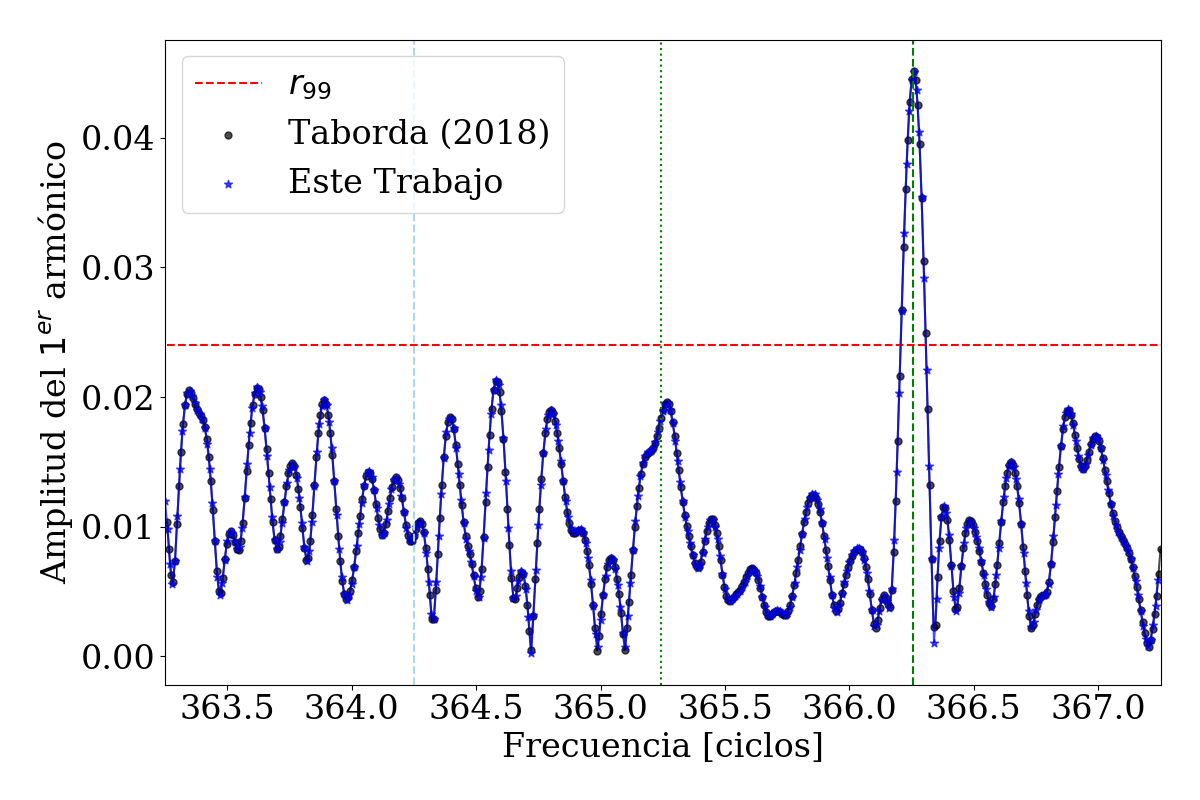
\includegraphics[width=0.75\linewidth]{sin_pesos_referencia_8_EeV.png}
        \caption{Comparación entre los análisis de anisotropía hechos para el mismo conjunto de datos, con el código de \cite{taborda} y con el código escrito para este trabajo.}
        \label{fig:sin_pesos_referencia}
      \end{figure}



\chapter{Dipolo en el rango 1 EeV - 2 EeV}
\graphicspath{{6_Dipole_1-2_EeV/}}
\section{Características del conjunto de datos} \label{specs}

	Además de los filtros aplicados mencionados en la sección \ref{filtro}, se aplican filtros adicionales sobre la energía y el rango de tiempo. Para estudiar los eventos en esta sección, consideramos los eventos entre 1\,EeV y 2\,EeV de energía y que ocurrieron entre las 12:00:00 GMT del 1 de enero de 2014 y las 12:00:00 GMT del 1 de enero de 2020. Se centró en este rango de tiempo porque entre hasta fines del año 2013, la tasa de eventos estuvo por debajo de la media de los años siguientes como se muestra en la Fig.\,\ref{fig:rate_2020_AllTriggers}. Además que el registro de eventos más reciente al que se tuvo para hacer este trabajo termina el 1 de Enero del 2020  a las 11:59:43 GMT, además de para estudiar una cantidad entera de años, se optó por considerar los eventos desde el 1 de Enero del 2014 a las 12:00:00 GMT.

    \begin{figure}[H]
    	\centering
    	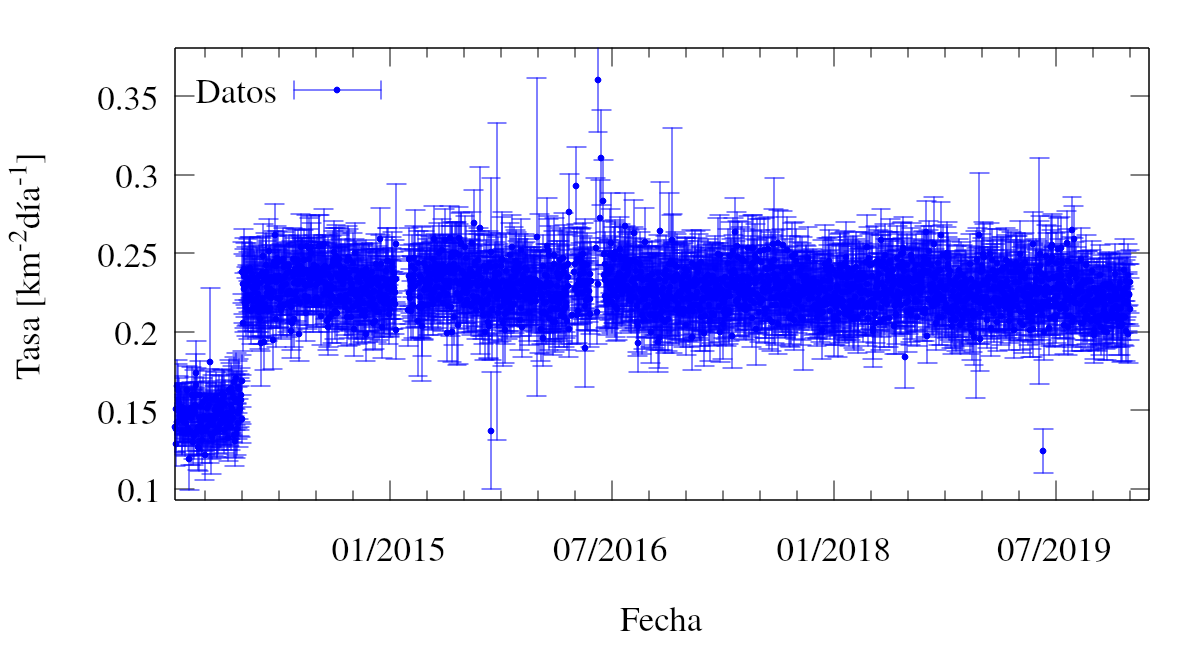
\includegraphics[width=0.75\textwidth]{rate_over_1-2_EeV-theta-60.png}
    	\caption{Tasa de eventos del conjunto más reciente de eventos con todos los disparos. Se observa un tasa baja en la segunda mitad del 2013.}
    	\label{fig:rate_2020_AllTriggers}
    \end{figure}

	Un resumen de todos los filtros aplicados se encuentra a continuación
		\begin{enumerate}
			\item Son eventos obtenidos mediante todos los disparos.
			\item Energía entre  [1 EeV , 2 EeV)
			\item Rango de tiempo:
			\begin{itemize}
				\item[-] Inicial:Jueves, 1 de Enero de 2014 12:00:00 GMT o 1388577600 UTC
				\item[-] Final:  Jueves, 1 de Enero de 2020 12:00:00 GMT o 1577880000 UTC
			\end{itemize}

		\end{enumerate}
	Aplicando estos filtros, se tienen $1\,081\,844$ eventos para estudiar en este rango de energía. 

    Se debe tener cuenta que el archivo de evento para todos los disparos tiene diferencias con el conjunto de eventos del disparo estándar. Porque el primero es entre los años 2013 y 2019 y el segundo se adquieren usando el disparo estándar entre los años 2004 y 2018.  Algo a considerar es que la colaboración cambió el algoritmo de reconstrucción de eventos en el 2019, con respecto a la versión del 2017.  

    En las  Figs.\,\ref{fig:deltaE} y \ref{fig:histograma} se muestra la diferencia entre las energías de la reconstrucción del año 2017 $E_{2017}$ de archivo de todos los disparos, que sigue sin ser corregida por los parámetros del clima, y la energía de último conjunto de datos $E_{2019}$, que ya fue corregida la modulación del clima y reconstruida por el nuevo algoritmo. Las variables utilizadas en las figuras son $\Delta E = E_{2019} - E_{2017}$ normalizada por la energía media $\langle E \rangle= (E_{2019} +  E_{2017})/2 $ para energías entre 1 EeV y 2 EeV de los dos conjuntos de datos. Se consideran eventos coincidentes entre las reconstrucciones del año 2017 y 2019. Puede apreciarse que la diferencia no esta centrada 0 y aparenta tener una modulación del clima. La amplitud de esta modulación es pequeña respecto al valor medio de $\Delta E$. Por lo tanto la diferencia entre ambos conjuntos se debe a una reconstrucción distinta de los eventos. 

        \begin{figure}[H]
          \centering
            \begin{subfigure}[b]{0.5\textwidth}
              \centering
              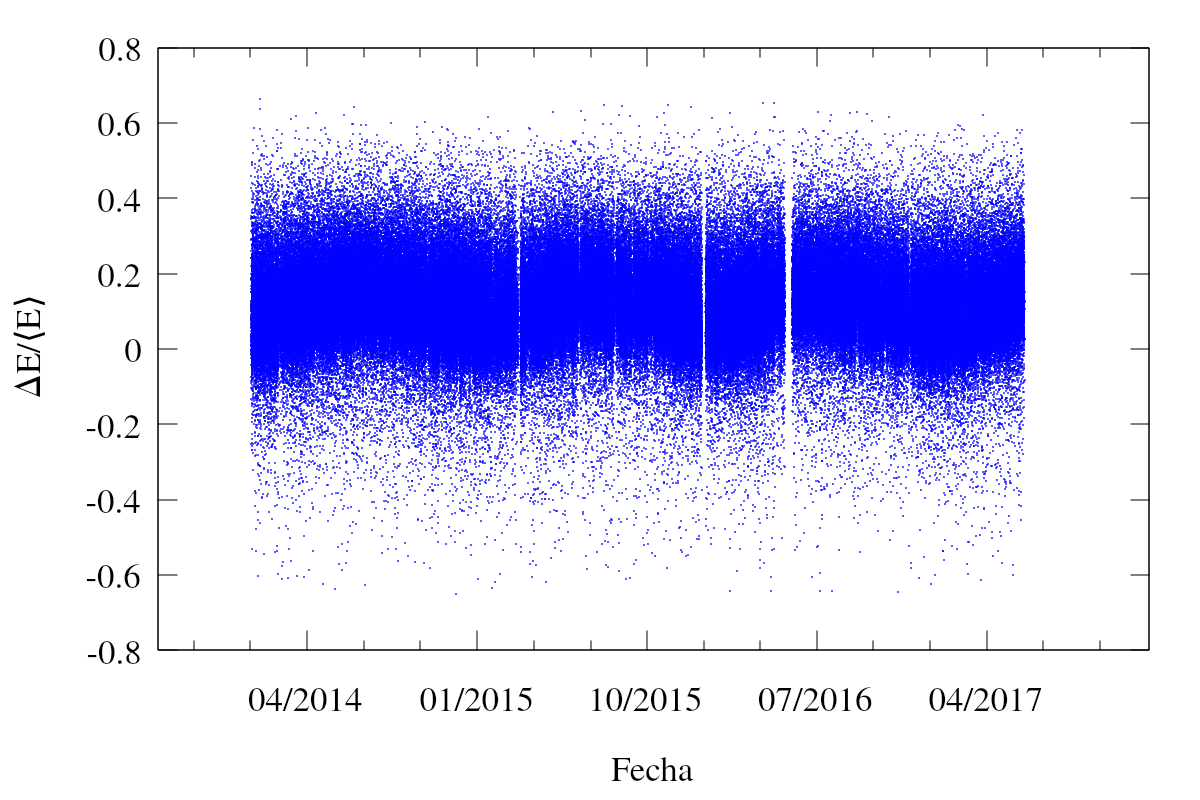
\includegraphics[width=\linewidth]{deltaE_tiempo_v2_rango_1_2.png}
              \caption{Diferencia entre las energías} \label{fig:deltaE}
            \end{subfigure}%
            \begin{subfigure}[b]{0.5\textwidth}
              \centering
              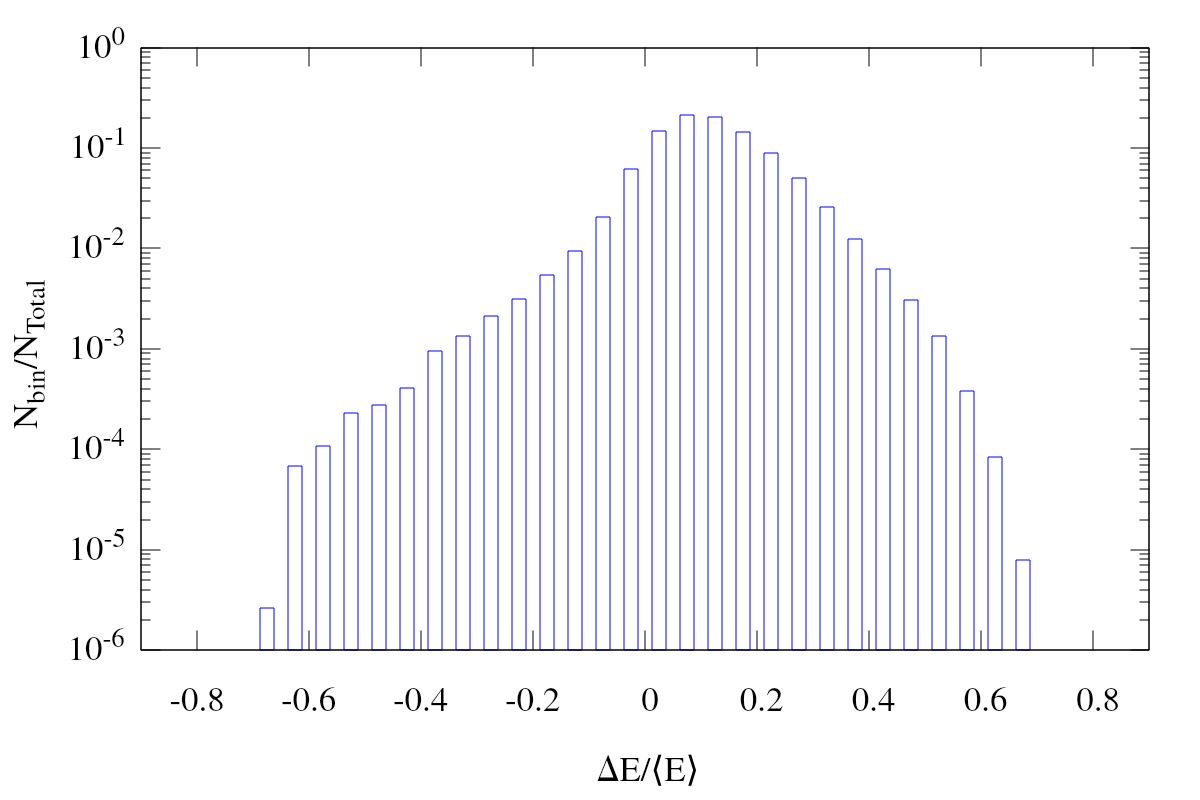
\includegraphics[width=\linewidth]{histograma_deltaE_v3_rango_1_2.png}
              \caption{Histograma de las diferencias}   \label{fig:histograma}
            \end{subfigure}
           \caption{Diferencia entre las energías de entre la reconstrucción del 2017 y del 2019}
         \end{figure}
	
\subsection{Pesos de los eventos para frecuencias de referencia}

En la Fig.\,\ref{pesos_bin_1_2} se muestran los valores de  $\Delta N_{cell,k}(\alpha^0)$ en función de la ascensión recta del cenit del observatorio, en el rango mencionado en la sección anterior \ref{specs}, para frecuencias de referencia. 
			 
			\begin{figure}[H]
				\centering
				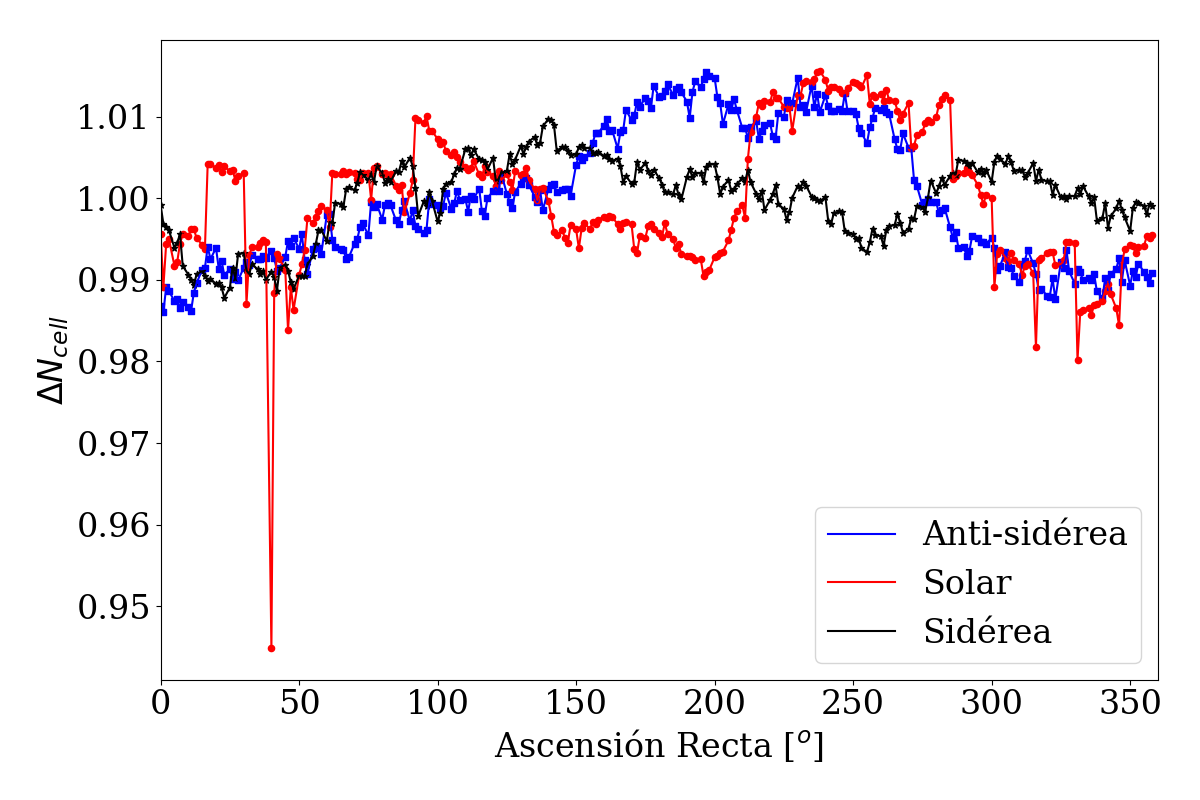
\includegraphics[width=0.6\textwidth]{weights_2013_2020.png}
				\caption{Variaciones de los hexágonos en función de la ascensión recta del observatorio para frecuencias características en rango mencionado. }
				\label{pesos_bin_1_2}
			\end{figure}


\section{Análisis de anisotropías en ascensión recta para el primer armónico}

En la Fig.\ref{anisotropia_rayleigh} se muestra en barrido de frecuencias para la amplitud del primer armónico de Fourier. Se marcan con líneas verticales las frecuencias de referencia mencionadas anteriormente. Se observa el barrido sin considerar las correcciones por las variaciones de los hexágonos con una línea discontinua. La  amplitud  en la frecuencia solar sin la corrección de los pesos es importante. Un ejemplo de errores sistemáticos puede ser que en épocas invernales el acceso a los tanques se dificulta y ponerlos en funcionamento nuevamente tras una tormenta o para un cambio de baterías puede llevar más tiempo que durante verano. 

		\begin{figure}[H]
			\centering
			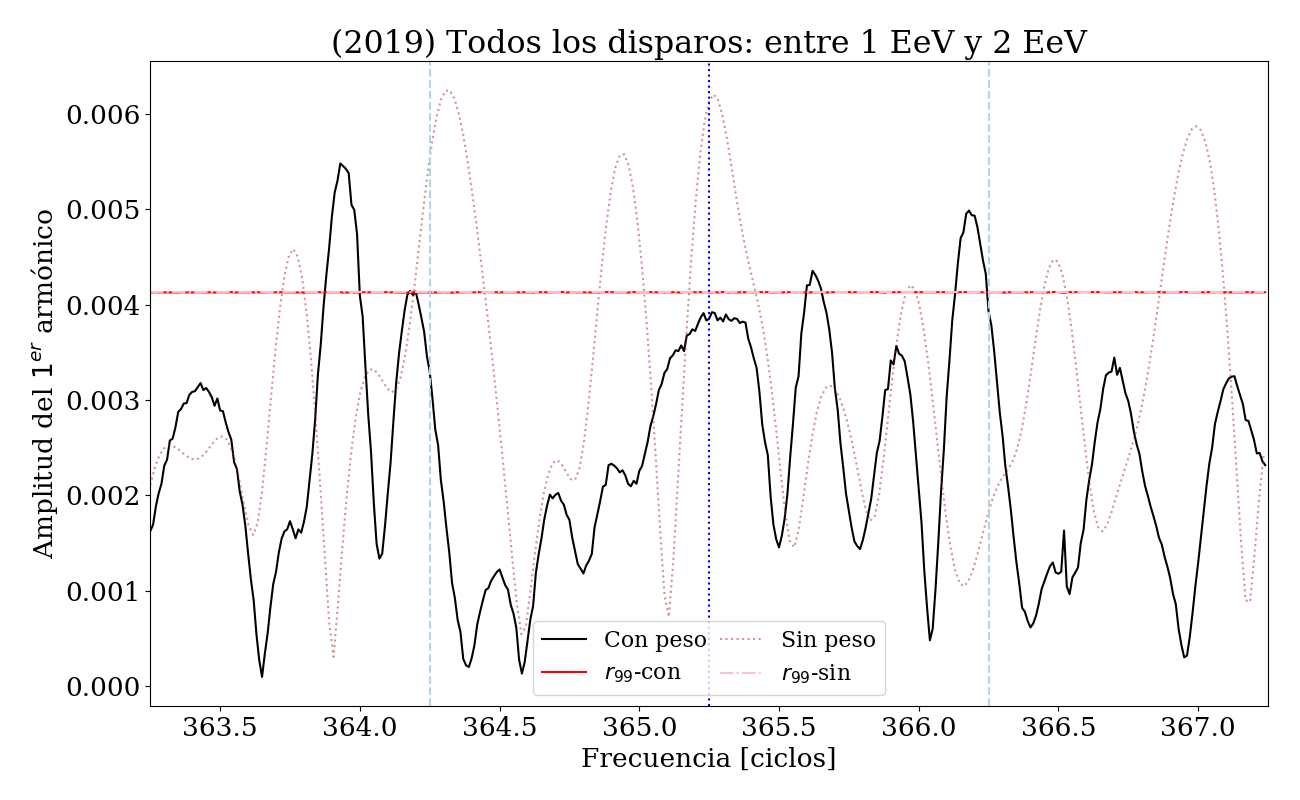
\includegraphics[width=0.85\linewidth]{pesos_sin_con_1_2_EeV.png}
			\caption{Anisotropía en función de la frecuencia para el rango de energía 1  EeV - 2 EeV. Se comparan los análisis sin los pesos y con los pesos de los hexágonos entre en 1 de Enero del 2014 y el 1 de Enero del 2020}
			\label{anisotropia_rayleigh}
		\end{figure}

Cuando se consideran los pesos, está amplitud disminuye y pasa a estar por debajo del umbral de $\tilde{r}_{99}$, y aparecen dos amplitudes por encima de este umbral: un pico es la frecuencia sidérea, donde buscamos las anisotropías en ascensión recta, y otro pico es cerca de la frecuencia anti-sidérea, que indica que existen componentes de errores sistemáticos sobre los datos que deben ser considerados. Por ejemplo, la corrección de clima que se analiza en el trabajo de licenciatura se realiza sobre el disparo estándar, se podría calcular los parámetros del clima utilizando los eventos de todos los disparos y comprobar si esto disminuye la amplitud del primer armónico de la frecuencia cercana a la anti-sidérea.

		
En la Tabla\,\ref{table:parametros_rayleigh} se resumen las amplitudes y fases obtenidas mediante el análisis a primer orden en Fourier. Se
		\begin{table}[H]
		\centering
		\begin{tabular}{|l|l|l|l|l|}
			\cline{2-5}
			\multicolumn{1}{c|}{} & \multicolumn{2}{c|}{Sin pesos} 		& \multicolumn{2}{c|}{Con pesos} \\ \hline
			Frecuencia:           & Solar          & Sidérea       		& Solar         & Sidérea        \\ \hline
			Fase $\phi$:          & $(251\pm13)^o$ & $(289\pm40)^o$		& $(288\pm20)^o$& $(337\pm19)^o$            \\ \hline
			Amplitud $r$:         & 0.0061         & $0.0018\pm0.0001$  & $0.0039\pm0.0001$      & $0.0040\pm0.0001$         \\ \hline
			$P(r)$:               & 0.0038 \%      & 41\%          		& 1.8 \%        & 1.3 \%       \\ \hline    
		\end{tabular}
		\caption{Comparación de los parámetros de fase y amplitud para las frecuencias sidérea y solar, analizando sin pesos y con los pesos de los hexágonos con el análisis de Rayleigh entre en 1 de Enero del 2014 y el 1 de Enero del 2020}
		\label{table:parametros_rayleigh}
		\end{table}


Las Fig.\,\ref{fig:bin_events_first_order} se muestra la tasa de eventos normalizada con pesos y sin pesos para este rango de energía. Las líneas discontinuas representan los parámetros de la Tabla\,\ref{table:parametros_rayleigh} para el primer armónico del análisis de Rayleigh de la frecuencia sidérea. Se observa que la modulación de los eventos con y sin pesos tiene características que la aproximación a primer orden no refleja. 	En las Fig.\,\ref{fig:bin_events_second_order_con} se muestra la tasa de eventos con pesos y el ajuste hasta el segundo orden en Fourier, en el mismo se muestra que este orden refleja mejor las características de los datos. Los resultados del análisis de Rayleigh  se muestran en la Tabla\,\ref{table:parametros_second_order}
	\begin{figure}[H]
		\centering
		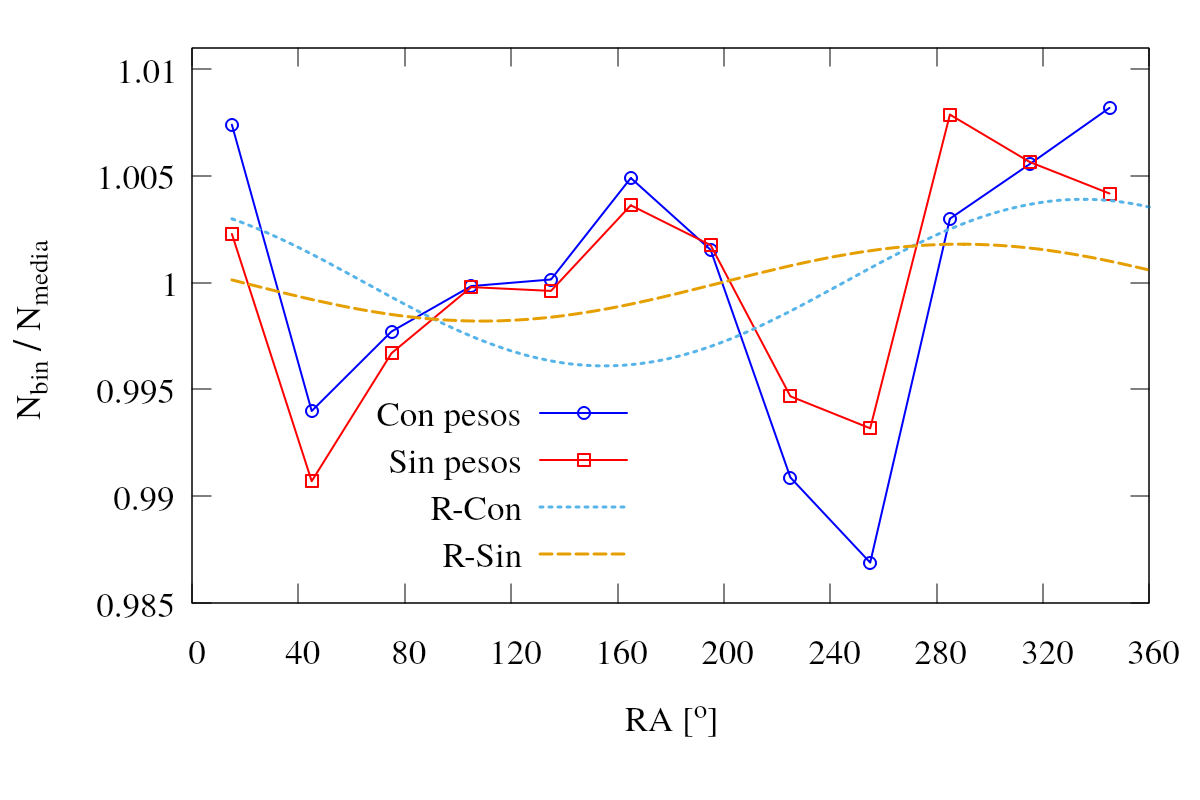
\includegraphics[width=0.65\linewidth]{eventos_clasificados_por_RA_v4.png}
		\caption{Distribución de la cantidad relativa de eventos en función de la ascensión recta a primer orden, en el rango de energía $1$ EeV - $2$ EeV.}
		\label{fig:bin_events_first_order}
	\end{figure}

        \begin{figure}[H]
          \centering
            \begin{subfigure}[b]{0.5\textwidth}
		\centering
		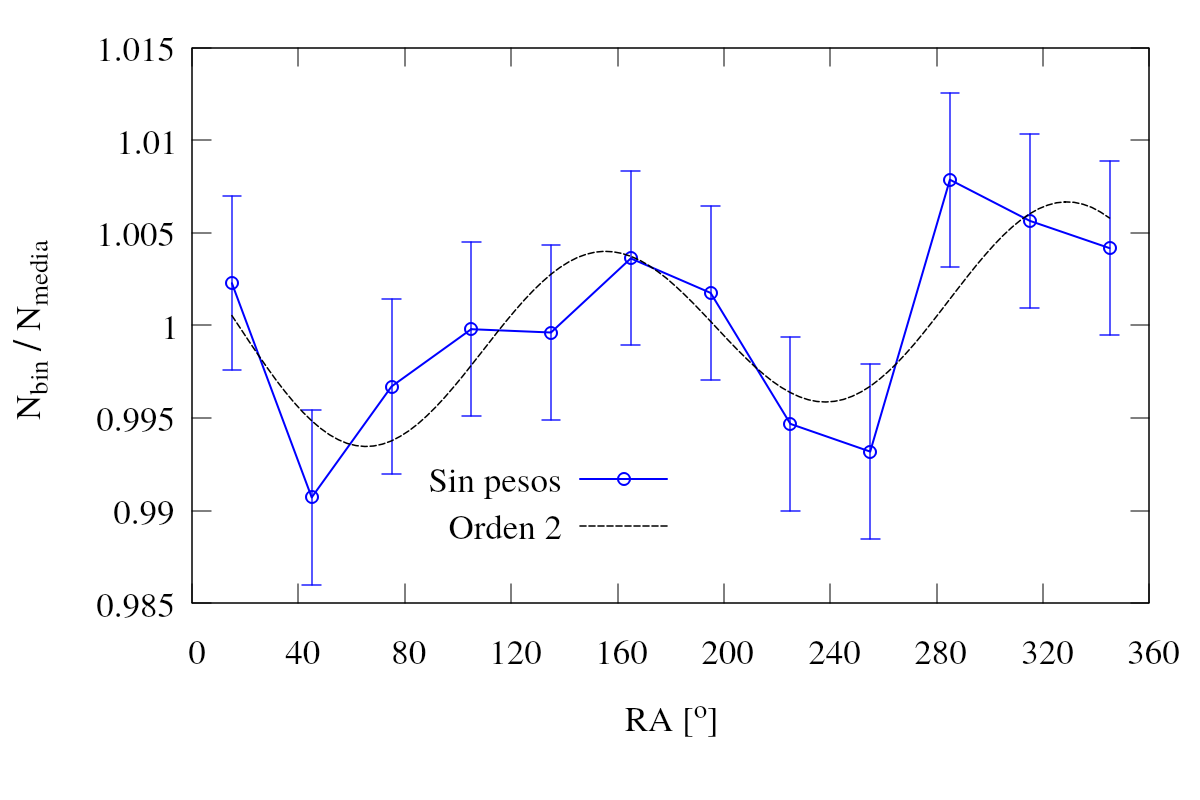
\includegraphics[width=\linewidth]{eventos_clasificados_por_RA_v7_orden_2_sin_pesos.png}
		\caption{Eventos sin pesos}		\label{fig:bin_events_second_order_sin}
            \end{subfigure}%
            \begin{subfigure}[b]{0.5\textwidth}
		\centering
		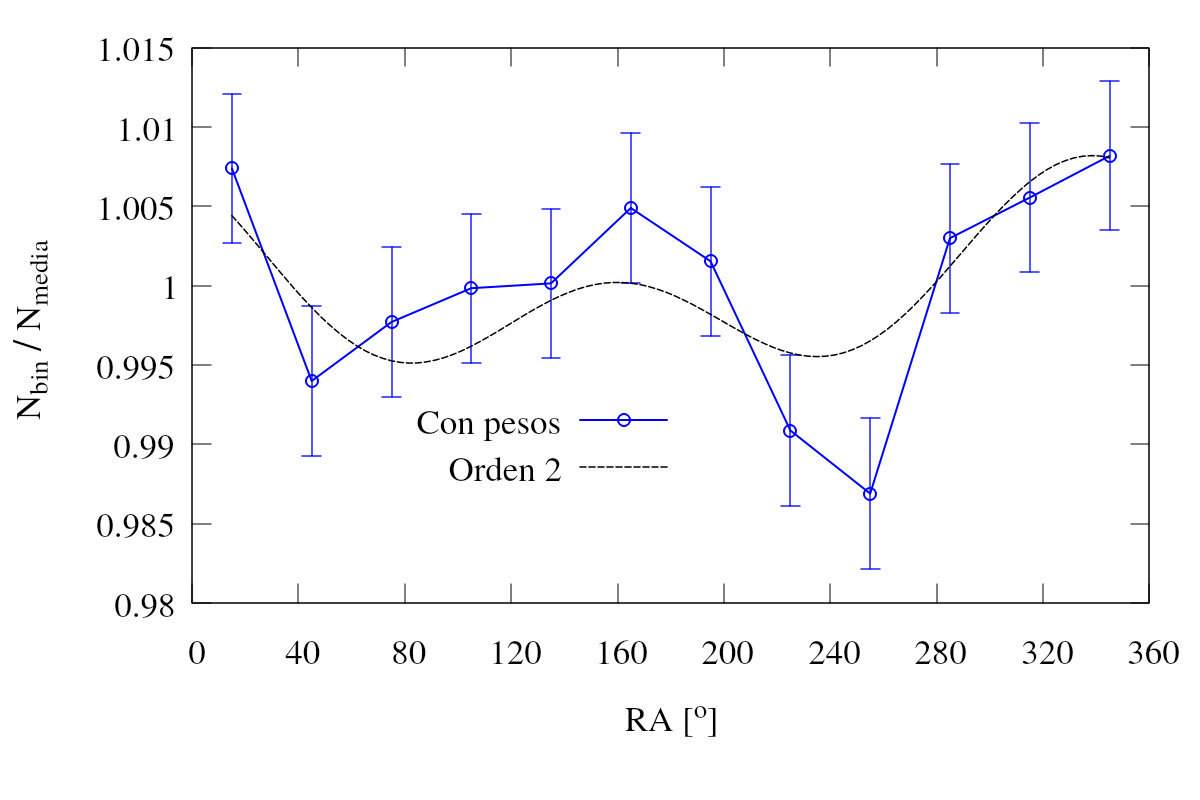
\includegraphics[width=\linewidth]{eventos_clasificados_por_RA_v7_orden_2_con_pesos.png}
		\caption{ Eventos con sus respectivos pesos}		\label{fig:bin_events_second_order_con}
            \end{subfigure}
           \caption{Distribución de la cantidad relativa de eventos en función de la ascensión recta a segundo orden en el rango de energía $1$ EeV - $2$ EeV entre en 1 de Enero del 2014 y el 1 de Enero del 2020.}
         \end{figure}

		\begin{table}[H]
		\centering
			\begin{tabular}{l|l|l|}
			\cline{2-3}
			                                      & Sin Pesos 		 & Con Pesos \\ \hline
			\multicolumn{1}{|l|}{Orden k :}       & 2                & 2                    \\ \hline
			\multicolumn{1}{|l|}{Fase $\phi_k$:}  & $(153\pm8)^o$    & $(170\pm9)^o$                   \\ \hline
			\multicolumn{1}{|l|}{Amplitud $r_k$:} & $0.0054\pm0.0001$& $0.0041\pm0.0001$               \\ \hline
			\multicolumn{1}{|l|}{$P(r_k)$:}       & $0.039$\%        & 1.0\%  \\ \hline
			\end{tabular}
		\caption{Parámetros obtenidos del ajuste a segundo orden con el análisis de Rayleigh.}
		\label{table:parametros_second_order}
		\end{table}

\subsection{Trabajo a futuro}

%Los resultados obtenidos en este rango de energía sugieren la existencia de un dipolo en ascensión recta, ligeramente corrido del centro galáctico que se encuentra alrededor de $260^o$, que proveería información sobre la transición galáctica - extra galáctica de las fuentes de los RCs de ultra alta energía.

La modulación del primer armónico de los eventos entre 1 EeV y 2 EeV tiene amplitudes por encima del umbral de $r_{99}$ para varias frecuencias, por lo que no puede decirse nada concreto sobre la existencia del dipolo en ascensión recta.


Durante el próximo semestre se trabajará en tratar de mejorar la calidad de los datos, en primer lugar implementando una corrección de los efectos climáticos a partir del conjunto de datos con todos los disparos.
%Para confirmar o desmentir  esto, durante el siguiente semestre trabajará en corregir la modulación del clima sobre los eventos, y verificar si el pico cercana a la frecuencia anti-sidérea que está por encima del umbral de $r_{99}$ puede disminuir.



\appendix
\chapter{Cosas para hacer:  Mails con Mollerach y correcciones}
% Fecha: 13/05/2020

% \begin{itemize}
% 	\done Para calcular los coeficientes del weather, queremos los mejores eventos, asi que tambien se usan solo los 6T5 (no es tan importante ganar un poquito mas de estadistica arribade 4 EeV para eso).

% 	\done En resumen usa los cortes 6T5 y $\theta<60$ para anisotropias y para weather correction.

% 	\done El corte de quality weather flag solo se usa para seleccionar los eventos para calcular las correcciones del weather.

% 	\done Los resultados nuevos son un poco raros, en siderea desaparecio toda la señal cuando pones pesos 1, y despues crece algo con los pesos. Revisa con los cortes bien puestos.

% 	\done Pone una tabla con amplitud y fase con y sin peso tambien.
% \end{itemize}


% Fecha: 20/05/2020

% \begin{itemize}

% 	\done Una cosa que se me ocurre es que al plot de hexagonos en frecuencia siderea le fitees un coseno. De ahi saca la amplitud del primer armónico de la modulación y la fase en RA donde esta el maximo.

% 	\done Despues hace el analisis de anisotropia en los eventos sin pesos y con pesos, y obtene la amplitud de la modulación y las fases del máximo en ambos casos.

% 	\done De ahi podriamos ver comparando las cantidades vectoriales (no solo la amplitud de la modulacion sino para donde apunta) qué es lo que esta pasando.

% 	\done Haceme un mail con esos resultados cuando los tengas, a ver si entendemos eso.
% \end{itemize}


Fecha: 27/05/2020

% \begin{itemize}
% 	\done los eventos son los 6T5 con cenit < 60 grados? Cuantos eventos son? (Pone siempre esos datos asi se sabe de quienes hablas)
% 	\done En la parte que fiteas el coseno, estas dejando libre una frecuencia, w en tu formula? 
% 	\done Lo que es relevante en el analisis que hacemos es el primer armonico de la funcion, aunque no de un buen fit. lo que afecta el valor del dipolo va ser la amplitud y fase en 1+A*cos(RA-B). Proba hacer ese fit y reporta los valores de A y B
% 	\done Otra cosa, no entiendo porque la figura de hexagonos y la de pesos tienen el maximo y minimo en los mismos valores. Los pesos son proporcionales a la inversa de los hexagonos.
% 	\done Porque no es periodica
% \end{itemize}


% Fecha: 28/05/2020

% \begin{itemize}
	% \done llama la atencion la modulacion de los hexagonos y de los pesos que pones en la tabla 1.3. Deberian tener aprox la misma amplitud y fase opuesta. Creo que estan mal los valores del fit a los hexagonos, deberia ser a ojo una amplitud cerca a 0.0035 y una fase cerca de 100. Igual es raro porque las curvas en el plot tienen pinta razonable. Fijate que cuando fiteas un coseno 1+A*cos(RA-B) va con menos B, asi B es la fase donde la funcion tiene el maximo. Fijate que si fiteas a una funcion con media distinta de 1, la amplitud es el factor A en C*(1+A*cos(RA-B)) y  no el factor  A en C+A*cos(RA-B)

	% \item 
	el test que queriamos hacer para ver si son compatibles las amplitudes de Fourier del primer armonico con y sin peso con la modulacion de los pesos no estaria funcionando. La idea es que si sumas vectorialmente un vector con amplitud igual a amplitud del primer armonico sin pesos apuntando en la direccion de la fase sin pesos mas otro vector con amplitud igual a la del fit a los pesos de los eventos apuntando en la fase del maximo del coseno, el vector suma deberia tener amplitud igual a la amplitud del analisis de fourier con pesos y apuntar en la direccion de la fase de ese analisis. No se en cual de los pedazos estara el error.
	
	% \item Para ir chequeando todo podrias:

	% \begin{itemize}
	
	% 	\done  binear los eventos en RA, por ejemplo en bines de 10 grados. 
		
	% 	\done Plotear el numero de evento en cada bin dividido la media (esta va a ser Ntotal/36) en funcion de la RA. 
		
	% 	\done Fitearle un coseno 1+A*cos(RA-B) a ese plot, te deberia dar aprox lo mismo que hacer el analisis de Fourier de los eventos sin peso. Asi podes comprobar si ese analisis te esta dando bien. Ademas es lindo hacer el plot y mostrar la distribucion en RA de los eventos.

	% 	\done  despues haces lo mismo poniendole los pesos a los eventos y comprobas si estas haciendo bien el analisis de Fourier con pesos.
	
	% 	\done  Me acabo de acordar que en algun momento tenias un lio con el  cero de donde contar la ascencion recta. Asegurate que los pesos los estas poniendo con la fase correcta, o sea que el tiempo sidereo en el que pones los hexagonos se corresponde bien con la RA del cenit del observatorio en ese momento (me parece que el problema podria venir de un corrimiento del cero, ya que eso da un error en la fase de los hexagonos)
	% \end{itemize}
%\end{itemize}


% Fecha: 09/06/2020

% Hay algunas cosas, al menos de notación, que  seria bueno mejorar y ver que no esten afectando los resultados.

% \begin{itemize}
	% \item
	% \done No cambies la notación de los papers de Auger( y la tesis de Oscar) para evitar confusiones. En particular, siguiendo la numeracion de tus puntos:

	% \begin{itemize}
	% 	\done 1 - periodo T: aca pones el periodo en segundos de la frecuencia que queres estudiar? por ejemplo para solar 24x3600? y para siderea 24x3600*365.25/366.25?

	% 	\done 2 - hora local se entiende la hora del reloj en Malargue. Mejor usa t en vez de hora local, aclarando que es el utc del evento (no tiene que estar entre 0 y 24 hs)

	% 	\done - Parece que estas intercambiando lo que normalmente se entiende como frecuencia y lo que se entiende como periodo:
	% 	\item

	% 		\begin{itemize}

	% 			\done la frecuencia solar equivale a $\sim$ 365,25 ciclos por año, y el periodo es la duracion de cada ciclo, y siempre se denoto con T, asi que seria mas correcto definir la coordenada angular asociada a cada frecuencia f\_x (sol, sid, antisid,..., con periodo T\_x), medida por ejemplo en horas,  como 

	% 			$h_x= 24 \frac{t-t_0}{T_x} + h_x(t_0)$

	% 			(en tu ecuacion parece estar al reves, o sea $T_x$ multiplicando, fijate si esta bien en el programa)

	% 			\done  para el grafico de las amplitudes para distintas frecuencias no importa el valor de $h_x(t_0)$, solo que tiene que ser consistente el valor para los hexagonos y los eventos, asi que ahi eventualmente podes tomar simplemente$ h_x=24  t/T_x$  (si queres el resultado en horas, yo te aconsejaria ponerlo directamente en radianes para el analisis de Fourier, reemplazando 24 por 2 pi)

	% 			\done Si queres calcular la fase siderea, sí es importante que h\_sid coincida con el right ascension, y sabemos que el right ascension del zenith vale  31.4971 grados para t0=1104537600 sec  (donde t es el UTC).

	% 			\done Del mismo modo para solar podrias ver cual es la hora solar en Malargue para un dado utc conocido (por ejemplo son las 21hs para las 0GMT de un dia particular)

	% 		\end{itemize}

	% 	\done 3 - En este punto decis que tomas el mod dado que T/Tsolar podria ser mayor que 1 y por eso $h_x$ podria ser mayor a 24. No importa cual sea el cociente entre los periodos, $h_x$ siempre va a llegar a valores MUCHO mayores que 24 porque t dura varios años (tu comentario me hace preocupar si en la ecuacion para h estabas realmente poniendo la hora local, entre 0 y 24) 

	% 	(esto lo estaba haciendo para el deltaN)

	% 	\done 4 - es confuso llamar peso whex a la modulacion en los hexagonos, siempre se llamo w a la inversa de eso, o sea el factor de peso para los eventos. Mejor llamalo delta N 

	% \end{itemize}

	% \done Para el analisis de Fourier valen los mismos comentarios

	% \done Cuando tengas los resultados de solar y siderea, con y sin pesos, mandalos, despues hay que revisar que los resultados del barrido en frecuencia coincida en esos dos casos.

	% \end{itemize}


Fecha  15-06-2020

\begin{itemize}
	\item Es que cada evento va pesado con los hexagonos del momento en que el evento fue registrado. El RA del cenit de Malargue en ese momento te dice cual es la correspondencia con el bin de los hexagonos que hay que usar. No se puede a ojo sumar o restar 2hs o lo que sea.
	\item A lo mejor no te estoy entendiendo bien lo que decir de las 2hs que agregaste, pero no hay nada arbitrario en la frecuencia siderea, hay que poner todo consistentemente.
\end{itemize}


\begin{biblio}
	\bibliography{mibib}
\end{biblio}

\end{document}